
% Chapter 2
\chapter{The \lhcb Detector}
\label{lhcb_detector}

The \lhcb experiment is an international collaboration located in the {\it European Organization for Nuclear Research}, \cern.
There are four major experiments at that location; Two of them, \atlas and \cms, are general purpose experiments whereas the other
two \alice and \lhcb, are dedecated to {\it heavy ion} and {\it flavour} physics respectively\footnote{\color{red} Flavour physics is  defined in and heavy ion in thsi sitation.}.
{\color{red} citation of the experiments}. All of the above experiments aim at detecting, recording and analysig as many as
posible high energy particle collisions, which are provided by the {\it Large Hadron Colider}, \lhc.
The latter is the world's most powerful particle accelerating machine built so far.
The \lhc machine accelerates, stores and colides two beams of protons. It is also capable of handling
heavy ion beams, \eg led, thus serving the physics program of the \alice experiment.
In both cases storage is achieved by magnetically forcing the beams to follow an eliptical trajectory.
The two beam trajectories are designed such that they colide with each other at four specific {\it interaction points},
where each of the four experiments is located. The \lhc accelerator as well as the four previously mentioned
experiments are located located about $100\m$ udnerground, to protect human population from radiation.
Given the complexity and techinical dificulties, building, operating and maintaining all these machines
is a remarkable achievement of human claboration.

\begin{figure}[t]
  \centering
  \includegraphics[width=\textwidth]{Figures/Chapter2/detector_cross_cmyk}
  \caption{Crossesctional view of the \lhcb detector. {\color{red} Steal picture from Roel, it is much better}}
  \label{lhcb_detector_cross_section}
\end{figure}

As mentioned in the previous paragraph the \lhcb experiment is dedeicateed to study falvor physics, see \secref{}.
The design of the \lhcb detector is optimized for this particular kind of physics.
Specifically, the experiment focuses in detecting \B mesons, explained in \secref{}. The latter type of
meson contains a \bquark quark which originates from a proton-proton colision. In \figref{} it can be seen
that \bquark quarks produced in such a colision, cluster mainly along the proton beam axis. In other words
roughly $50\%$ of the \bquark quarks {\it fly} inside a region of $\sim 45^\circ$ solid angle along both
directions of the beam axis. This region is also called {\it forward} region. The design of \lhcb detector,
shown in \figref{}, is such that it exploits this special production feature of \bquark quarks. Implying that
a $4\pi$ detector geometry like the rest of the \lhc experiments, where the center of colision is sourounded
by layers of detectors, is not necessary. Instead the the \lhcb detector covers the forward region along one
of the two directions of the beam axis, impliyg that roughly $25\%$ of the b quarks produced are detectable
by \lhcb. This forward design allows for increased purity of the recorded \B mesons at the expence of a limited
physics program compared to the rest of the \lhcb experiments.

The full \lhcb detector specifications, designs and performance are described in {\color{red} detector paper \cite{jnst}}.
The aproach of the current chapter is to very briefly address the function and perfromance of the detector components
throughout \secref{det_tracking} - \secref{det_calo}. Emphasis, is given to these sub-detectors that are relevant
to the analysis performed in \chapref{Data_Analysis} as well as to the trigger system which is of crucial importance
to efficiently running the \lhcb experiment.

\begin{figure}[t]
  \centering
  \includegraphics[width=0.8\textwidth, trim=0cm 0cm 0cm 2.5cm, clip=true]{Figures/Chapter2/08_rad_acc_scheme_right}
  \caption{bb quark pair production.}
  \label{bb_roduction_angles}
\end{figure}


\section{Tracking Systems}
\label{det_tracking}
The tracking sub-detectors are responsible for registering spacial coordinates of charged particles.
The coordinates from multiple layers of tracking sub-systems are processed by the tracking algorithms
to produce {\it tracks}, which are objects representing the trajectory of a charged particle. There are
three distinct tracking sub-detectors in \lhcb shown in \figref{lhcb_detector_cross_section}; Closest to the interaction point is
the {\it VErtex LOcator}, \velo, then just before the \lhcb magnet is the {\it Tracking Turisensis}, \ttracker,
and  lastly the {\it Outer Tracker} \ot. There are several track types that are {\it reconstructed} by
the tracking algorithms, depending on which of the tracking sub-detectors provided information to produce
the track object. The varius track types are shown in \figref{track_types}. The most common tracks used are {\it long}
which have the highest momentum resolution. The overal reconstruction efficiency of long tracks is $\sim 96\%$.

\begin{figure}[t]
  \centering
  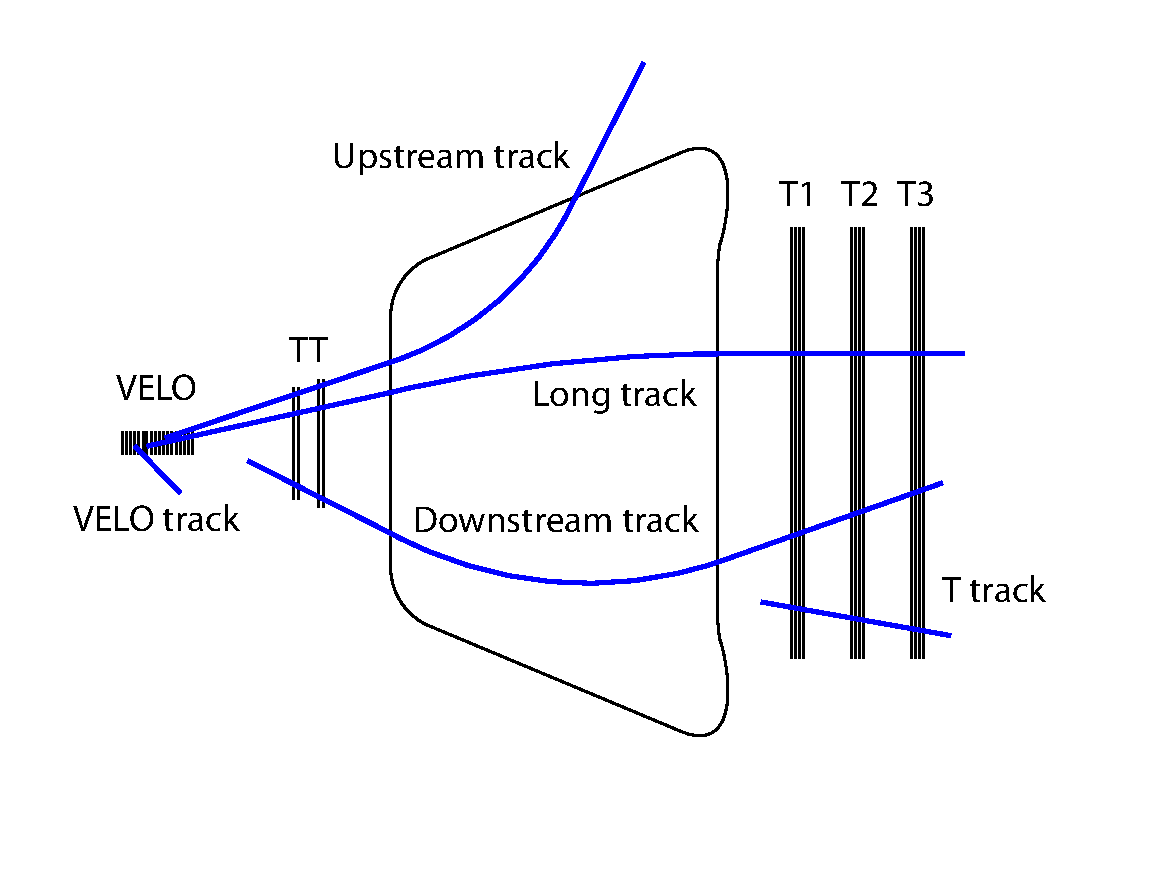
\includegraphics[width=0.7\textwidth]{Figures/Chapter2/trackTypesRunIAndII}
  \caption{\lhcb track types.}
  \label{track_types}
\end{figure}

A charged particle that traverses the \lhcb magnet is deflected. The amount of deflection is inversly proportional
to its momentum. The latter is exploited by tracking algorithms to estimate the momentum of a track. The relative
momentum momentum resolution of the tracking sytem, shown in \figref{det_deltappvp}, is $\nicefrac{\Delta p}{p} \sim 0.5 \%$
for low mementum tracks and up to $1\%$ for 200\gevc momentim tracks. Intuitively, tracks that do not deflect a
lot have inferior momentum resolution.

Measuring the mass of a particle, like the \Bs meson, is achieved by combining tracks in order to build a complete
cascade of partcile decays (also refered to as {\it decay chanell}). The mass measurement presicion varies depending
on the specific decay chanell. Two body \B decays including a \jpsi have the most precise mass resolution of about
$8 \mevcc$. On the other hand decay chanells including neutral particles, \ie $\Bs\to\phi\gamma$, have a worst resolution of
about $100 \mevcc$. Note that neutral particles are undetected by the tracking system. Instead the calorimetry,
introduced in \secref{det_calo}, system is responsible for reconstructing these type of particles.

\begin{figure}[t]
  \centering
  \begin{subfigure}{0.5\textwidth}
    \raggedright
    \includegraphics[width=\textwidth]{Figures/Chapter2/dppVsp-crop-cmyk}
    \caption{}
    \label{det_deltappvp}
  \end{subfigure}%
  \begin{subfigure}{0.5\textwidth}
    \raggedleft
    \includegraphics[width=\textwidth]{Figures/Chapter2/DataResXY_1PV_2012-crop-cmyk.pdf}
    \caption{}
    \label{det_velo_pv_res}
  \end{subfigure}
  \caption{ trigger scheams.}
  \label{det_velo_perf}
\end{figure}

Certain important analysis performed with the \lhcb detector rely on measuring the {\it flight distance} of a particle, like the \Bs meson.
Flight distance is typically the distance between the point were the two protons colideed, called {\it Primary Vertex} (PV)
and the point were the \Bs, in that case, decayed. This last point is called {\it Secondary Vertex} (SV). The \velo sub-detector
was designed for optimum spacial resolution, by placing the \velo sensors as close to the beam as posible, $\sim 8 \mm$.
The PV position resolution depends strongly on the number of tracks used to build the vertex and can be seen in \figref{det_velo_pv_res}.
Measuring the flight distance translates to a {\it decay time} time measurement. The latter is the time interval between
the production and decay of a particle and it is the actual quantity that a typical {\it time dependant} analysis,
\eg \BsJpsiPhi, requires. The average decay time resolution measured with the above channel is $\sim 45\fs$, which
implies that the \phis measurement discussed in \secref{measuring_phis}, is indded posibe to perform.

Lastly, a big part of the \lhcb physics program includes muons. The muon system cositis of {\it Multi Wire Proportional Chambers}
(MWPC). It is positioned after the calorimeters, with the exception of the first, M1, muon station.
Note that muons can penetrate through a large volume of led, like the one present in the calorimeter system,
without decaying. There are 5 muons stations in total; Each station is devided in 4 concentric regions.
The granularity\footnote{In this context granularity is essentially the distance between the wires of the MWPC.}
of each station becomes progresively smaller as one moves towards the inner regions which are closer to the beam pipe.
This is done to acount for the increasing track density that is typicaly found in the forward region. This way
the special resolution is higher exactly where it is needed. The $x$ coordinate hit resolution in all regions
is superior comapred to the $y$ coordinate; Since the configuration direction of the \lhcb magnetic field streangth
is such that tracks bend only along the $x$ plane. The $(x,y)$ resolution varies from $(4,10)\mm$ to $(150,180)\mm$
respectivelly fro the inner M1 region and the outer M5 region. The overal detector efficiency is $\>98\%$.


\section{Particle Identification}
\label{det_pid}

The kaons and pions are idistiguishable in the absence of dedicated particle identification, {\it PID}, detectors. 
Furthermore, a particle that is not stopped by the calorimeters is most likely identified as a muon, 
since muons can penetrate the entire \lhcb detector without decaying. In addition, properly identifing 
electrons, photons and pions is a chalenging task that require sophisticated setup and algorithms.
These experimental dificulties are tackeled by exploiting information from several sub-detector systems;
thus increasing the purity of the analyzed data. 

The two {\it Cherenkov} based PID sub-detectors in \lhcb, \richone and \richtwo, amied at identifying low and 
high momentum tracks respectively. The way the \rich systems provide particle identification information is 
based on the velocity measurement implied by the angle of emmission of a Cherenkov radiation. 
The muon system also plays a role in PID. The presence of hits in the muon stations that 
could be ascocaited to a certain track increse the probability that this track corresponds to real muon, 
see \chapref{Muon_id_hlt} also. Lastly, the calorimeter systems aim at increasing the chances of correctly 
identifieng electrons, photons and pions, as mentioned in \secref{det_calo}.
Further details regarding the PID performance of \lhcb can be found in the overall detector \cite{Aaij:2014jba}, 
\rich system \cite{Adinolfi:1495721}, \muonID \cite{Archilli:1553139} performance studies respectivelly.  

%% \begin{table}[!h]
%%   \center
%%   \begin{tabular}{c c c}
%%     \hline
%%       particle      & $\epsilon_{\rm PID}$  & given mis-id probability \\
%%      \hline
%%       $\electron$   &  $90\%$  & $\sim 5\%$    \electron - hadron  \\
%%       $\kaon$       &  $95\%$  & $\sim 5\%$    \pion - \kaon       \\
%%       $\mmu$        &  $97\%$  & $\sim 1-3\%$  \pion - \mup        \\
%%       \hline
%%   \end{tabular}
%%   \caption{\small Nominal efficiencies of the PID system. The mis-id probabilities quoted in the third
%%            column are required for the efficiency computation. }
%%   \label{pid_efficiencies}
%% \end{table}


\section{Calorimetry}
\label{det_calo}
Calorimeters in \lhcb measure the energy of particles provided that all of the subsequent particle decays are
contained withing the calorimeter. Furthermore in the case of netrual particles, like photons or \piz,
calorimeters are the only mean with which these netrual particles can be detected; since the tracking system
only detect charged particles. There are four relevant sub-detectors
that enable proper calorimetry at \lhcb. First the combination of the {\it Scintillating Pad Detector} (\spd)
and the {\it Pre Shower} (\presh) detectors with a lead layer in-between them enables to distinguish \piz from
photons, and photons from electrons which leave the same signature in the electromagnetic calorimeter.
Subsequently the electromagnetic, \ecal, and hadronic, \hcal, calorimeters measure the energy of photons
and neutral hadrons respectively. The calorimeter system is not explicitly used in the analysis of \chapref{Data_Analysis}.
However, they are implicitly used since information from the \spd and \presh sub-detectors are used
by the \lzero trigger system to estimate the overall {\it multiplicity} of an event. Multiplicity essentialy
provide a quick estimate, to the \lzero trigger system, on wheather a certain event is intrasting from physics
point of view. Furthermore, the lead material that is interlayered between the \ecal and \hcal active detector material,
stops\footnote{Stop in this context means that the particle decays and all its decay products are contained inside the calorimeter
volume, such that energy of the initial particle is estimated.} most of the hadrons and thus preventing them
from being mis-identified by as muons by the subsequent muon stations.

\section{The trigger system}
\label{det_trigger}
The trigger system is responsible for keeping the amount of data that the detector writes to offline storage
at a manageable level, since it is not feasible to save every event. The three levels of the \lhcb trigger system
are able to quickly, $\sim 25\ns$, decide weather a certain collision, {\it event}, is interesting from physics point
of view and should thus be written out to storage. The criteria used to filter out the interesting events, get
progressively more stringent at each trigger level. The whole trigger chain is optimized for maximum
signal purity given the amount of computing and storage infrastructure. In more detail the first trigger
level, \lzero, reads the detector at a rate of $40\mhz$, while the subsequent {\it Higher Level Trigger},
\hltone and \hlttwo, write out to storage at $5\khz$. The first trigger level is a pure hardware
implementation whilst the other two are software only.

\begin{figure}[t]
  \centering
  \begin{subfigure}{0.5\textwidth}
    \raggedright
    \includegraphics[width=\textwidth]{Figures/Chapter2/LHCb_Trigger_RunIAlgDetail_May2015}
    \caption{}
    \label{det_run_one_trigger}
  \end{subfigure}%
  \hfill%
  \begin{subfigure}{0.5\textwidth}
    \raggedleft
    \includegraphics[width=\textwidth]{Figures/Chapter2/LHCb_Trigger_RunII_May2015}
    \caption{}
    \label{det_run_two_trigger}
  \end{subfigure}
  \caption{ \runone (left) and \runtwo (right) trigger system schemes.}
  \label{det_trigger_scheams}
\end{figure}

The organization of the trigger system is done in {\it streams} and {\it trigger lines}.
The four streams, {\it Hadron}, {\it Muon}, {\it DiMuon} and {\it Photon}, correspond to the possible
ways that an event can be pass through the \lzero trigger level. Complicated selection criteria are
not affordable from computation power point of view at this stage, since the $40\mhz$ input rate of \lzero is quite
big. After the rate is reduced by $\sim 1$ order of magnitude the data are fed to the subsequent
higher level trigger, where tracking and PID information become available. The \hltone and \hlttwo
trigger levels organize their output in trigger lines. Essentially, each trigger line is a collection
of selection criteria similar to the ones applied during the offline data analysis, but looser.
Furthermore, the trigger lines are software implementations and can thus be quite general as to what
they trigger on, or on the other hand they can be very dedicated.

The overall performance of the \lhcb trigger system is $\sim 90\%$ for dimuon channels and $\sim 30\%$ for
multi-body hadronic final states. A complete performance study of the trigger system can be found in chapter
5 of \cite{Aaij:2014jba}. The current section focuses on the trigger performance involving muons;
The corresponding efficiencies are shown in \figref{det_run_one_muon_line_eff}.

\begin{figure}[t]
  \centering
  \begin{subfigure}{0.5\textwidth}
    \raggedright
    \includegraphics[width=\textwidth,trim=0.45cm 0cm 0.4cm 0cm, clip=true]{Figures/Chapter2/l0_muon_eff}
    \caption{}
    \label{det_run_one_l0_muon_line_eff}
  \end{subfigure}%
  \hfill%
  \begin{subfigure}{0.5\textwidth}
    \raggedleft
    \includegraphics[width=\textwidth,trim=0.45cm 0cm 0.4cm 0cm, clip=true]{Figures/Chapter2/hlt1_muon_eff}
    \caption{}
    \label{det_run_one_hlt1_muon_line_eff}
  \end{subfigure}%
  \hfill%
  \begin{subfigure}{0.5\textwidth}
    \raggedright
    \includegraphics[width=\textwidth,trim=0.45cm 0cm 0.4cm 0cm, clip=true]{Figures/Chapter2/hlt2_muon_eff}
    \caption{}
    \label{det_run_one_hlt2_muon_line_eff}
  \end{subfigure}
  \caption{\runone muon line efficiencies of the \lzero (A), \hltone (B) and \hlttwo (C) trigger stages.}
  \label{det_run_one_muon_line_eff}
\end{figure}

Lastly there are two more worth mentioning features of the \lhcb trigger system. First is the so called
{\it deferral} trigger, where $20\%$ of the data triggered by \lzero are temporarily stored and proceed by the \hltone
during the periods where the \lhc does not provide colliding beams and thus the \lhcb computing infrastructure
would normally idle. This effectively increases the amount of available computing power which can be used
to improve other features of the trigger system. The second interesting feature is the novel technique of
{\it online detector alignment and calibration} that was enabled in view of the \runtwo, see \cite{Aaij:2016rxn}.
The technique makes it possible that the output data quality of the trigger becomes identical to the offline data quality.
This means that offline data analysis can be performed straight from the output of the trigger, which saves
a lot of computing resources, accelerates the analysis and minimizes the chances of introducing mistakes.


\section{The \BJpsiKst Decay in \lhcb}
\label{BspsiKst_at_lhcb}

The \BsJpsiKst process is a typical channel for which the \lhcb has a high detection efficiency.
The presence of muon in the final state yields a high trigger efficiency, while the intermediate
\Kstarz resonance decays within the \velo into a \Kp and a \pim thus resulting in two Long tracks.
Thanks to PID information and the optimized selection described in \secref{det_pid} most of the bakcground
is filtered out. The only difficult point is the low branching fraction of the \BsJpsiKst decay
compared to the \BdJpsiKst whose invariant mass is very close to the one of the \BsJpsiKst, see \secref{mass_BDTG_selection}.
Thus, special care needs to be taken when modeling the mass distribution of these two channels.
The total \BsJpsiKst yield accumulated over the full \runone is about 1800 signal candidates, see \equref{signal_yields}.
An \lhcb event is shown in \figref{det_evt_display}. A reconstructed \BsJpsiKst decay candidate is shown in
more detail in \figref{det_jpsikst_cand}.

\begin{figure}[t]
  \centering
  \begin{subfigure}{\textwidth}
    % \raggedright
    \includegraphics[width=\textwidth]{Figures/Chapter2/top}
    % \caption{}
    \label{det_evt_display_top}
  \end{subfigure}
  \begin{subfigure}{\textwidth}
    % \raggedleft
    \includegraphics[width=\textwidth]{Figures/Chapter2/side}
    % \caption{}
    \label{det_evt_display_side}
  \end{subfigure}
  \caption{Horizontal (top) and vertical (bottom) cross section of an \lhcb event.
           Straght lines indicate Long tracks; where kaons, pions, muons, protons and electrons
           are represented with red, orange, green, magenta and blue color respectively. \ecal and \hcal energy depositions
           are shown as blue and orange bars respectively; the length of each bar is proportional to the energy deposited.
           Muon hits are illustrated with green blocks.}
  \label{det_evt_display}
\end{figure}

\begin{figure}[t]
  \centering
  %\begin{turn}{90}
 \includegraphics[width=1\textwidth,trim=0cm 0cm 17cm 0cm, clip=true]{Figures/Chapter2/jpsikst_event.pdf}
  %\end{turn}
  \caption{A \BsJpsiKst candidate. The purple and cyan circles correspond to the primary and secondarry
           vertices respectivelly. The dashed cyan line, is not an actual track; it illustrates the \Bs flight distance.
            Black lines represent \velo tracks and colored lines indicate particles as in \figref{det_evt_display}.
            Note how \velo tracks apear to originate from the primary vertex. Also note the how \Bs final state tracks
            ({\color{green}\mmu},{\color{green}\mmu},{\color{red}\kaon},{\color{orange}\pion}) intersect at the secondary vertex.}
  \label{det_jpsikst_cand}
\end{figure}
